\thispagestyle{timhieukhoahocnone}
\pagestyle{timhieukhoahoc}
\everymath{\color{timhieukhoahoc}}
\blfootnote{$^1$\text{\color{timhieukhoahoc}Viện Khoa học Vật liệu, Viện Hàn lâm Khoa học và Công nghệ Việt Nam.}}
\graphicspath{{../timhieukhoahoc/pic/}}
\begingroup
\AddToShipoutPicture*{\put(0,616){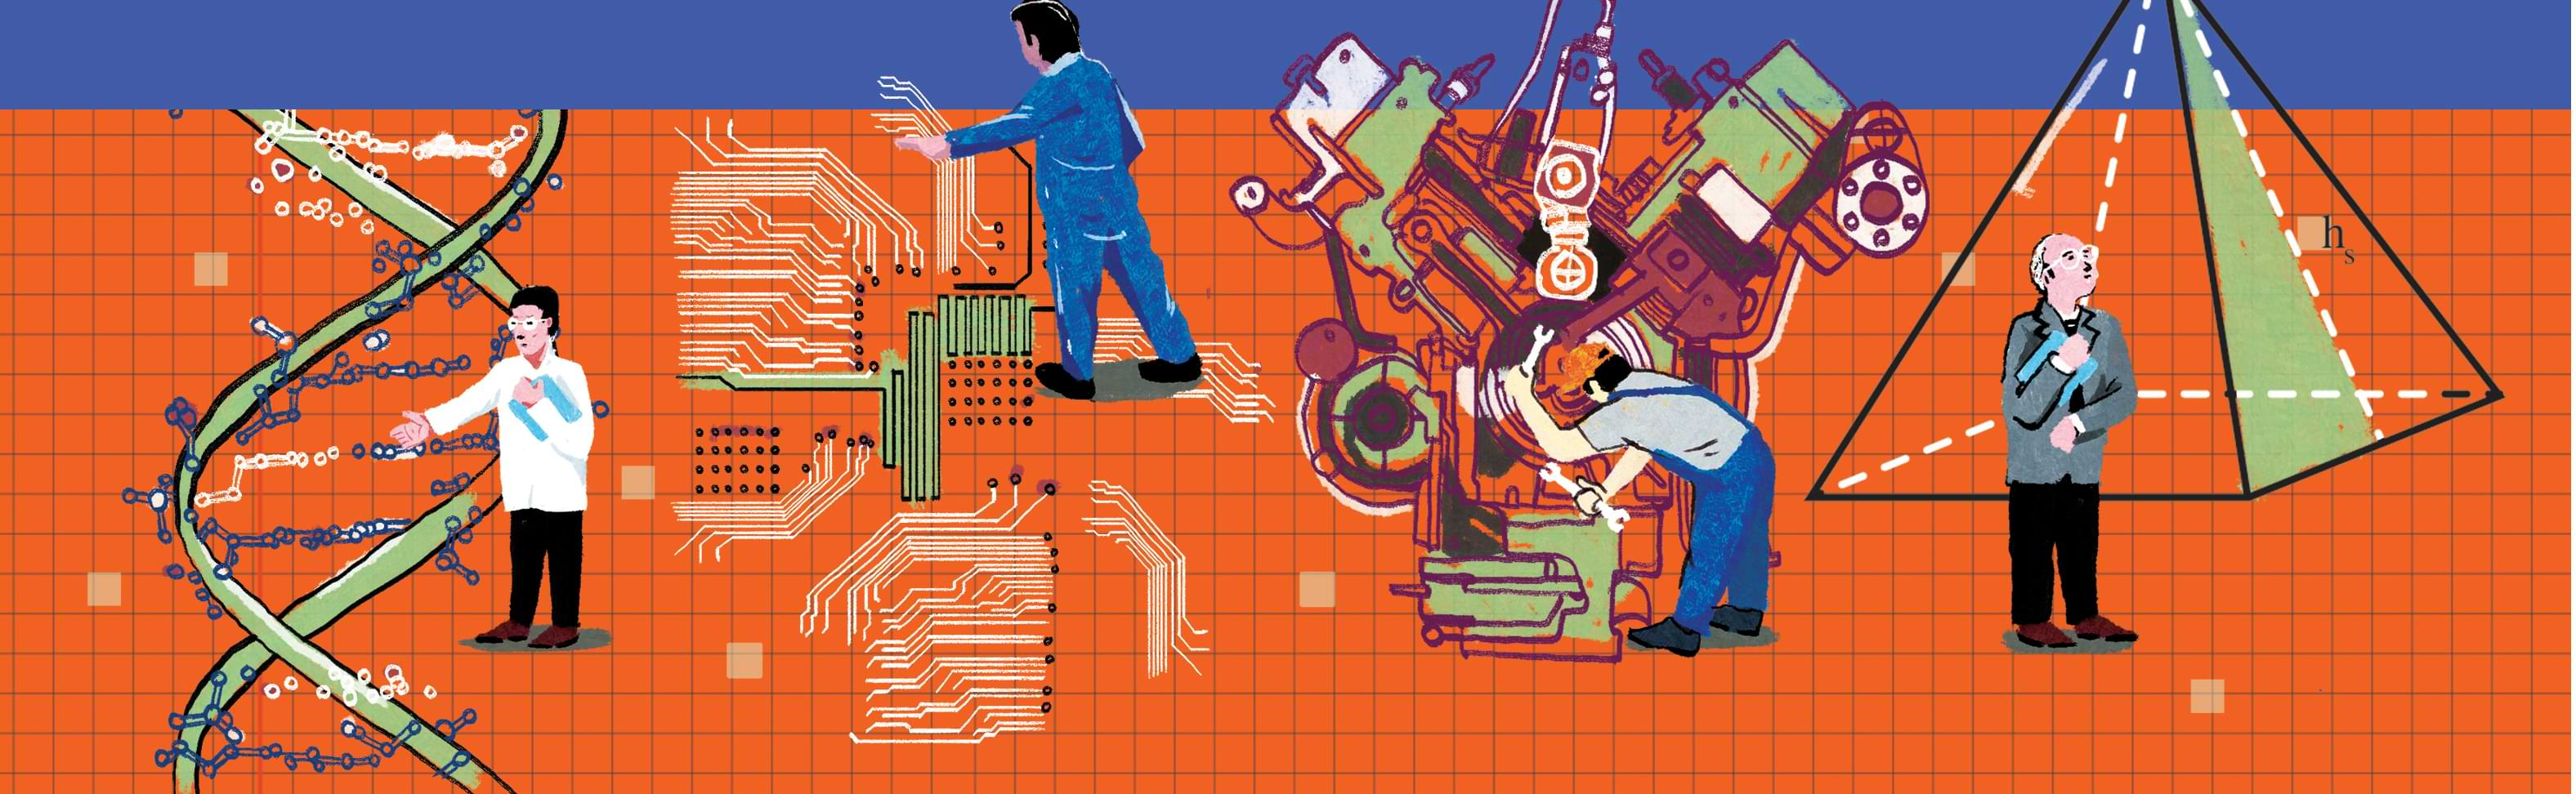
\includegraphics[width=19.3cm]{../bannertimhieu}}}
\AddToShipoutPicture*{\put(130,555){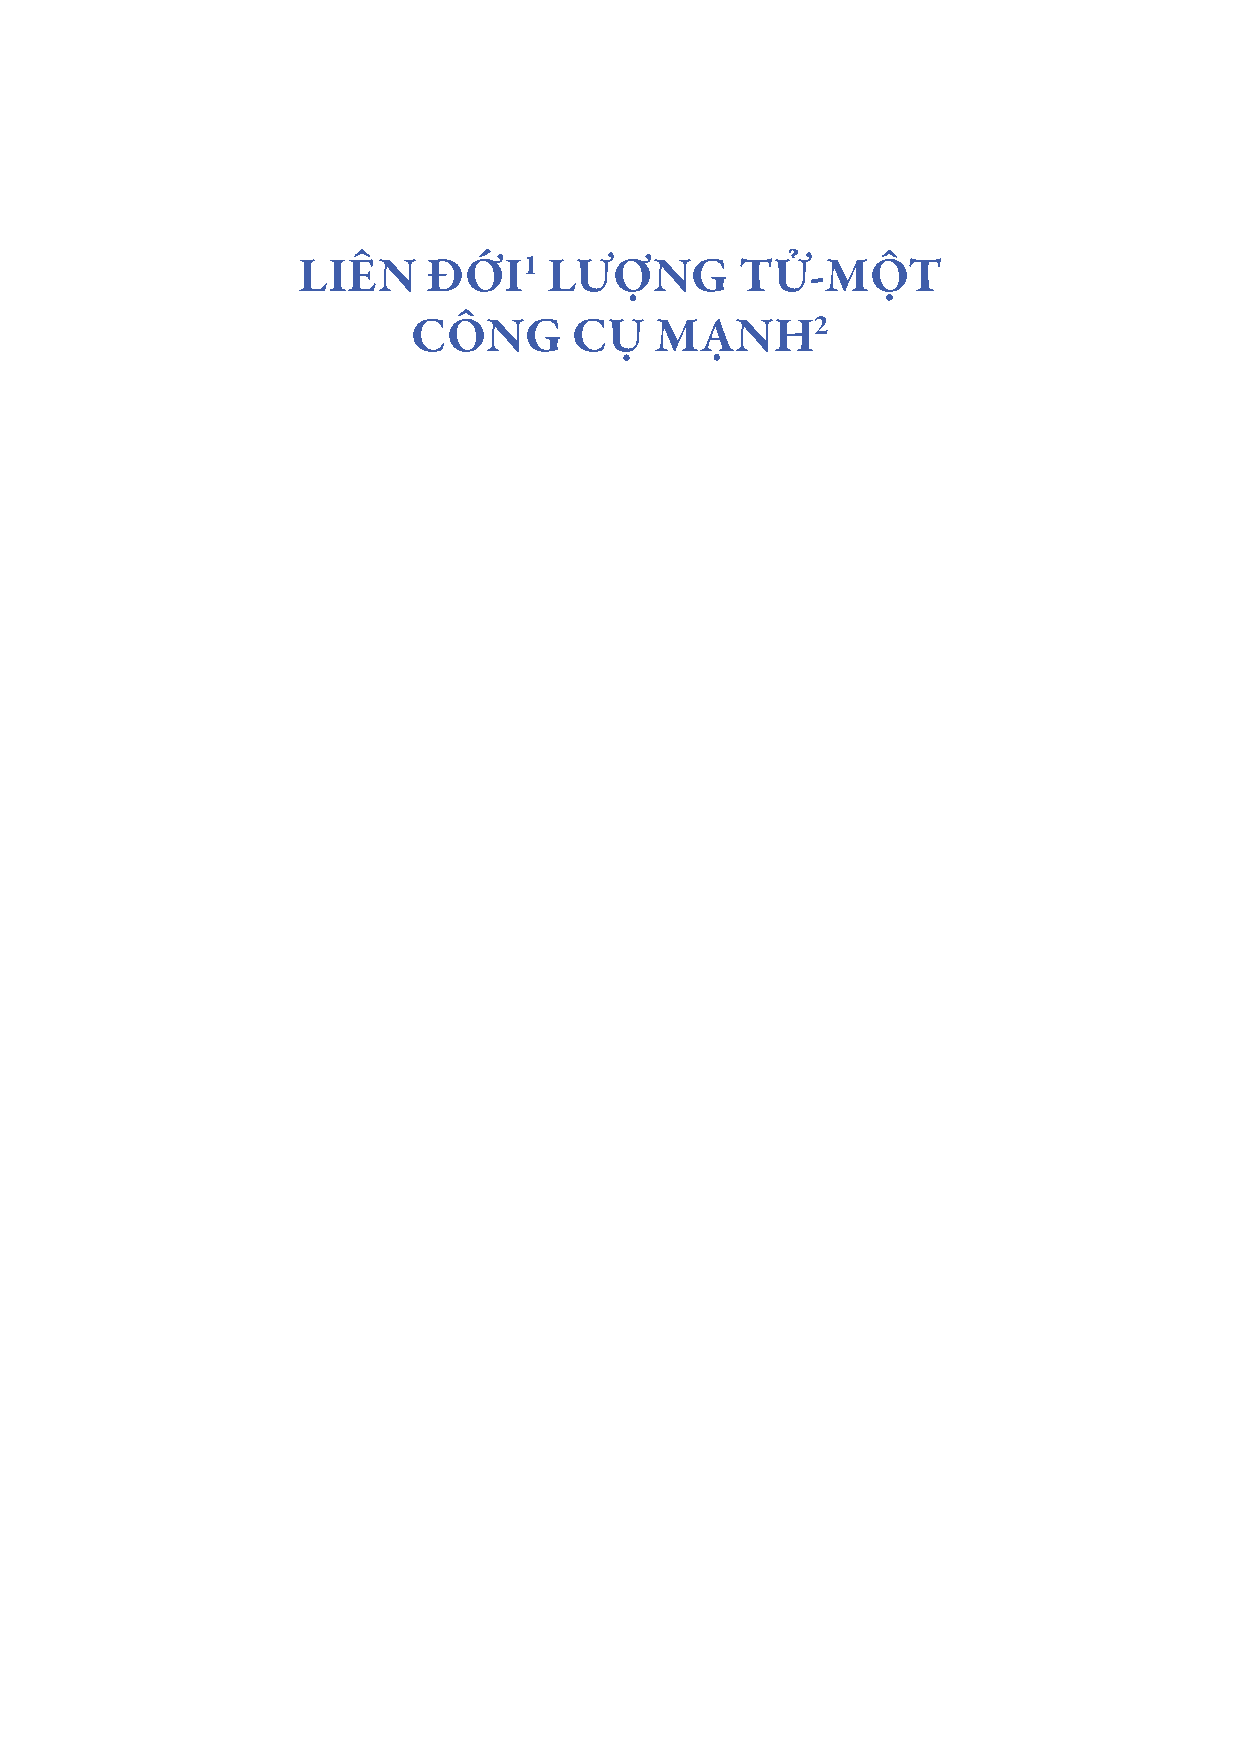
\includegraphics[scale=1]{../tieude.pdf}}}
\centering
\endgroup
\vspace*{155pt}

\begin{multicols}{2}
	Trái đất nơi chúng ta sống bao gồm không gian, vật thể, năng lượng, tất cả đều tương tác với nhau và biến đổi theo thời gian. Để có thể sống sót, sinh vật nào cũng cần nhận thông tin về thế giới bên ngoài thông qua các giác quan, trong đó thị giác là phức tạp và tinh vi nhất. Mắt là cửa ngõ của hệ thống thị giác, mắt có chức năng thu nhận hình ảnh thế giới bên ngoài nhờ có ánh sáng.
	\vskip 0.1cm
	Thật đáng ngạc nhiên và vô lý khi chúng ta hiểu biết quá ít về ánh sáng và mắt. Bạn thử nhớ lại xem, chúng ta đã học cách sử dụng ánh sáng, hệ thống thị giác và mắt được bao nhiêu? 
	\vskip 0.1cm
	$\pmb{1.}$ \textbf{\color{timhieukhoahoc}Ánh sáng là gì?}
	\vskip 0.1cm
	Trong bài này, chúng ta hiểu ánh sáng là cảm thụ khi chùm photon với bước sóng thích hợp rơi vào võng mạc. 
	\begin{figure}[H]
		\vspace*{-5pt}
		\centering
		\captionsetup{labelformat= empty, justification=centering}
		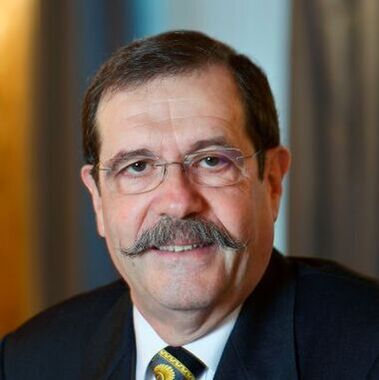
\includegraphics[width= 1\linewidth]{1}
		\caption{\small\textit{\color{timhieukhoahoc}Hình $1$. Bầu trời ban ngày có góc khối bằng $2\pi sr$.}}
		\vspace*{-10pt}
	\end{figure}
	Ánh sáng từ nguồn sáng chiếu vào các vật thể, tương tác với chúng, sau khi đi vào mắt, đem thông tin về thế giới bên ngoài cho chúng ta. Não bộ tiếp nhận, xử lý và ghi nhận luồng thông tin thị giác này để đảm bảo cuộc sống của chúng ta. Thị giác của chúng ta đã tiến hóa qua hàng triệu năm trong môi trường chiếu sáng tự nhiên, nhưng chiếu sáng nhân tạo đang tạo ra các biến đổi sâu sắc đến hệ thống thị giác.
	\vskip 0.1cm
	$\pmb{2.}$	\textbf{\color{timhieukhoahoc}Môi trường chiếu sáng.}
	\vskip 0.1cm
	Ánh sáng tự nhiên chủ yếu đi từ mặt trời, và được tán xạ trên bầu trời, tạo ra một quang cảnh đẹp lộng lẫy và một hệ sinh thái vô cùng hiếm hoi cho muôn loài phát triển.
	\vskip 0.1cm
	Bầu trời trên trái đất có góc khối $2\pi sr$, và có sự trùng hợp kỳ lạ, võng mạc của chúng ta cũng có góc thu sáng khoảng $2\pi sr$. Mặc dù bầu trời không chói lóa, nhưng độ rọi xuống đất rất cao. Mặt trời rất chói, nhưng có góc phát sáng rất nhỏ. Tương tự như vậy, hốc mắt (\textit{fovea}) rất nhạy sáng trong góc thu sáng rất nhỏ. Trái đất tự quay nên ánh sáng thay đổi cường độ, màu sắc theo nhịp ngày đêm.
	\vskip 0.1cm
	$\pmb{3.}$	\textbf{\color{timhieukhoahoc}Mắt để làm gì?}
	\vskip 0.1cm
	Ai cũng biết mắt là để nhìn! Tuyệt đối đúng! Nhưng chưa đủ. Mắt có những $3$ chức năng.  
	\vskip 0.1cm
	Mắt nhìn là chức năng thị giác: phân biệt hình dạng, màu sắc, chất liệu, độ sáng, chuyển động và vị trí. Mắt còn điều chỉnh nhịp sinh học: ánh sáng gửi tín hiệu qua mắt đến đồng hồ trung tâm trong não, rồi ra lệnh cho hệ thống hormone điều chỉnh tâm trạng, sinh lý và giấc ngủ của chúng ta. Lạc nhịp sinh học gây ra rất nhiều bệnh tật, từ trầm cảm đến ung thư, từ mất ngủ đến béo phì. 
	\begin{figure}[H]
		\vspace*{-5pt}
		\centering
		\captionsetup{labelformat= empty, justification=centering}
		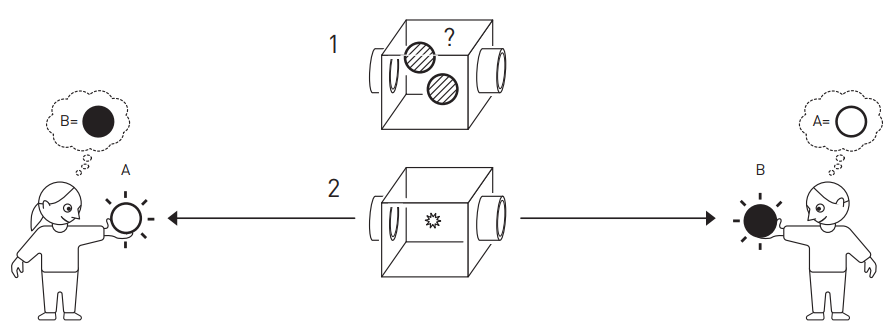
\includegraphics[width= 1\linewidth]{2}
		\caption{\small\textit{\color{timhieukhoahoc}Hình $2$. Mắt là của ngõ hệ thống thị giác.}}
		\vspace*{-10pt}
	\end{figure}
	Mắt còn là cửa sổ tâm hồn! đó là chức năng trao đổi cảm xúc? Giống loài nào cũng cần chọn bạn tình để sinh sôi. Họ thường nhìn vào mắt nhau. Không thích ai thì đừng cho họ nhìn sâu vào mắt mình nhé!
	\vskip 0.1cm
	$\pmb{4.}$ Mắt tinh vì có cấu trúc buồng tối. Phần lớn các loài động vật sở hữu một trong $2$ loại mắt, đó là mắt kép và mắt đơn với cấu trúc buồng tối. 
	\begin{figure}[H]
		\vspace*{-5pt}
		\centering
		\captionsetup{labelformat= empty, justification=centering}
		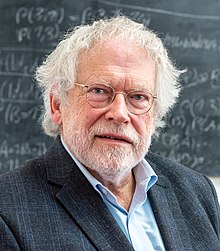
\includegraphics[width= 0.9\linewidth]{3}
		\caption{\small\textit{\color{timhieukhoahoc}Hình $3$. Mặt cắt nhãn cầu.}}
		\vspace*{-10pt}
	\end{figure}
	Mắt người có hai bộ phận quan trọng nhất, đó là nhãn cầu tạo ảnh và võng mạc thu ảnh. Nhãn cầu có đường kính khoảng $25$ mm được bao bọc bởi lớp củng mạc chắn ánh sáng. Phần trong suốt hơi lồi phía trước của nhãn cầu là giác mạc (Hình $3$). Lực khúc xạ của giác mạc là $40$ D, còn thủy tinh thể là $20$ D, nhỏ hơn lực khúc xạ của giác mạc nhưng lại đảm nhận vai trò điều tiết, tức là lấy nét. Phía trước thủy tinh thể là đồng tử, đồng tử điều chỉnh lượng ánh sáng rơi vào võng mạc.
	\vskip 0.1cm
	$\pmb{5.}$ \textbf{\color{timhieukhoahoc}Võng mạc.}
	\vskip 0.1cm
	Võng mạc là lớp phủ bên trong nhãn cầu, được cấu tạo bởi nhiều lớp tế bào với nhiều chức năng khác nhau. Võng mạc thu ảnh nhờ các loại tế bào quang thụ chuyển đổi kích thích thành tín hiệu thần kinh, gửi về não bộ. Có $120$ triệu tế bào que nhạy với ánh sáng yếu đề nhìn ban đêm và $7$ triệu tế bào nón, nhạy với $3$ dải bước sóng khác nhau khi ánh sáng mạnh. Tế bào nón tập trung chủ yếu tại hố mắt, nằm giữa hoàng điểm (Hình $4$). Tế bào nón gửi thông tin qua bó thần kinh thị giác cho não sau khi đã được xử lý sơ bộ. Võng mạc thực hiện việc nén tín hiệu khoảng $1000$ lần.
	\begin{figure}[H]
		\vspace*{-5pt}
		\centering
		\captionsetup{labelformat= empty, justification=centering}
		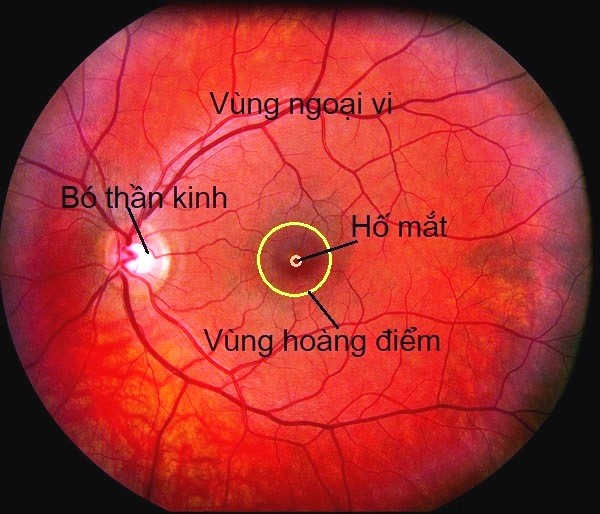
\includegraphics[width= 0.75\linewidth]{4}
		\caption{\small\textit{\color{timhieukhoahoc}Hình $4$. Ảnh chụp đáy mắt.}}
		\vspace*{-10pt}
	\end{figure}
	Bó thần kinh thị giác có hơn $1$ triệu sợi, truyền tín hiệu vào não bộ. Số lượng lớn các sợi thần kinh là rào cản cho việc thay thế võng mạc bằng các cảm biến nhân tạo vì không ghép nối được hết các điện cực trong một không gian nhỏ hẹp. 
	\begin{figure}[H]
		\vspace*{-5pt}
		\centering
		\captionsetup{labelformat= empty, justification=centering}
		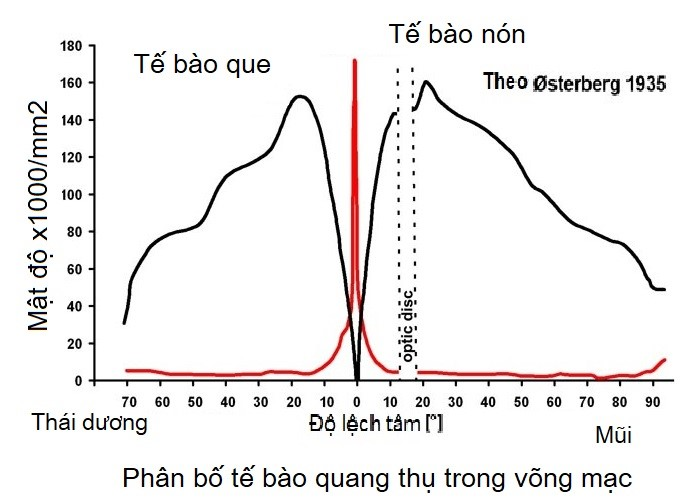
\includegraphics[width= 1\linewidth]{5}
		\caption{\small\textit{\color{timhieukhoahoc}Hình $5$. Phân bố tế bào quang thụ.}}
		\vspace*{-5pt}
	\end{figure}	
	Ban đêm, tín hiệu từ nhiều tế bào que tập hợp lại với nhau để tăng độ nhạy, nhưng giảm độ phân giải. Ta thấy trên Hình $5$, mật độ tế bào que phân bố rộng trên toàn bộ võng mạc, nhưng không có trong hốc mắt. Vì vậy bạn muốn rõ trong đêm thì đừng nhìn thẳng vào đối tượng! Tế bào nón tập trung chủ yếu trong hốc mắt nằm trong vùng hoàng điểm, là nơi có độ phân giải cao nhất. Khi đọc chữ, mắt luôn điều chỉnh sao cho ảnh của các chi tiết nhỏ nhất rơi vào hố mắt.
	\vskip 0.1cm
	$\pmb{6.}$ \textbf{\color{timhieukhoahoc}Mắt tạo ảnh thế nào?}
	\vskip 0.1cm
	Các tia sáng đi từ vật thể bên ngoài được khúc xạ bởi các bộ phận quang học của nhãn cầu, tạo hình ảnh lên võng mạc. Hình ảnh trên võng mạc là ảnh thực nhưng có chiều lộn ngược. Não sẽ làm nhiệm vụ đảo chiều. 
	\begin{figure}[H]
		\vspace*{-5pt}
		\centering
		\captionsetup{labelformat= empty, justification=centering}
		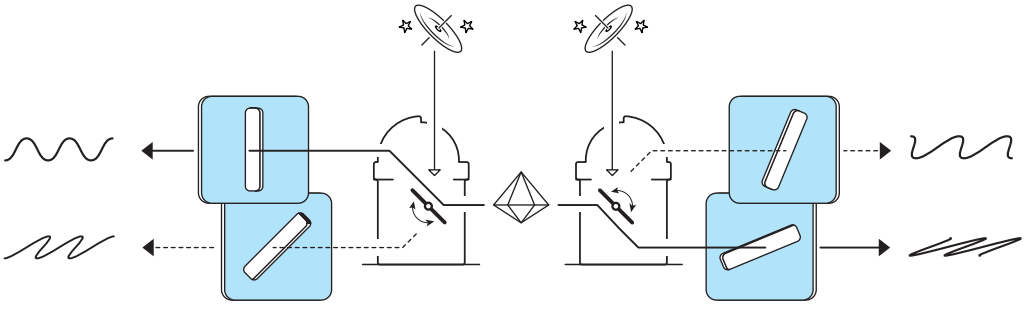
\includegraphics[width= 1\linewidth]{6}
		\caption{\small\textit{\color{timhieukhoahoc}Hình $6$. Sơ đồ tạo ảnh lên võng mạc.}}
		\vspace*{-10pt}
	\end{figure}
	Phần ngoại vi rộng khắp võng mạc có phân giải thấp, nhưng lại đóng góp chủ yếu vào việc điều chỉnh nhịp sinh học và kích thước đồng tử. 
	\vskip 0.1cm
	$\pmb{7.}$ \textbf{\color{timhieukhoahoc}Thị lực.}
	\vskip 0.1cm
	Khả năng phân giải theo góc của mắt gọi là thị lực, được đo bằng bảng thử thị lực. Thị lực $10/10$ có tương đương với khả năng phân biệt được $1$ phút cung ($1$ min). 
	\begin{figure}[H]
		\vspace*{-5pt}
		\centering
		\captionsetup{labelformat= empty, justification=centering}
		
\includegraphics[width= 1\linewidth]{7}
		\caption{\small\textit{\color{timhieukhoahoc}Hình $7$. Phổ hấp thụ tế bào quang thụ.}}
		\vspace*{-5pt}
	\end{figure}
	Thị lực là thước đo chất lượng thị giác của mỗi cá nhân, nhưng thị lực phụ thuộc vào môi trường chiếu sáng. Chiếu sáng tốt không những nâng cao thị lực, mà còn có tác dụng bảo vệ hoàng điểm khỏi tác động có hại của ánh sáng xanh. 
	\vskip 0.1cm
	$\pmb{8.}$ \textbf{\color{timhieukhoahoc}Màu sắc.}
	\vskip 0.1cm
	Khả năng phân biệt màu sắc của thị giác gọi là sắc giác. Nhờ có $3$ loại tế bào nón mà não bộ cảm nhận và phân biệt được rất nhiều màu và sắc (Hình $7$). Màu thay đổi chủ yếu do bước sóng đỉnh vùng thay đổi. Sắc độ tăng lên khi dải sóng kích thích hẹp lại.
	\vskip 0.1cm
	Khả năng phân biệt màu trong vùng tím cao hơn trong vùng xanh lá cây. 
	\begin{figure}[H]
		\vspace*{-5pt}
		\centering
		\captionsetup{labelformat= empty, justification=centering}
		
\includegraphics[width= 1\linewidth]{8}
		\caption{\small\textit{\color{timhieukhoahoc}Hình $8$. Không gian màu HSV.}}
		\vspace*{-10pt}
	\end{figure}
	Để thuận tiện cho việc ghi nhận và xử lý màu sắc, người ta đã xây dựng các không gian màu số hóa dựa trên kết quả cảm nhận của các người quan sát chuẩn. Ví dụ về không gian màu HSV được thể hiện trên Hình $8$.
	\vskip 0.1cm
	Tương phản màu sắc cũng đóng góp vào việc nâng cao nhận biết hình ảnh.
	\vskip 0.1cm
	$\pmb{9.}$ \textbf{\color{timhieukhoahoc}Trường nhìn.}
	\vskip 0.1cm 
	Mắt bồ câu và mắt các động vật bị săn mồi nằm ở hai bên đầu, có trường nhìn $2$D rất rộng, chủ yếu để phát hiện kẻ săn mồi. Mắt cú vọ tập trung ở phía trước, tạo ra trường nhìn lập thể $3$D, hẹp nhưng xác định khoảng cách rất chính xác để vồ mồi. 
	\vskip 0.1cm
	Mắt người có trường nhìn ngang vừa rộng, vừa sâu (Hình $9$), nhưng chỉ nhìn rõ ở khu vực trung tâm. Con người vừa là kẻ săn mồi, vừa là con mồi. Có nhiều người bị hỏng thị giác ngoại vi, trường nhìn thu hẹp, tham gia giao thông rất nguy hiểm. 
	\begin{figure}[H]
		\vspace*{-5pt}
		\centering
		\captionsetup{labelformat= empty, justification=centering}
		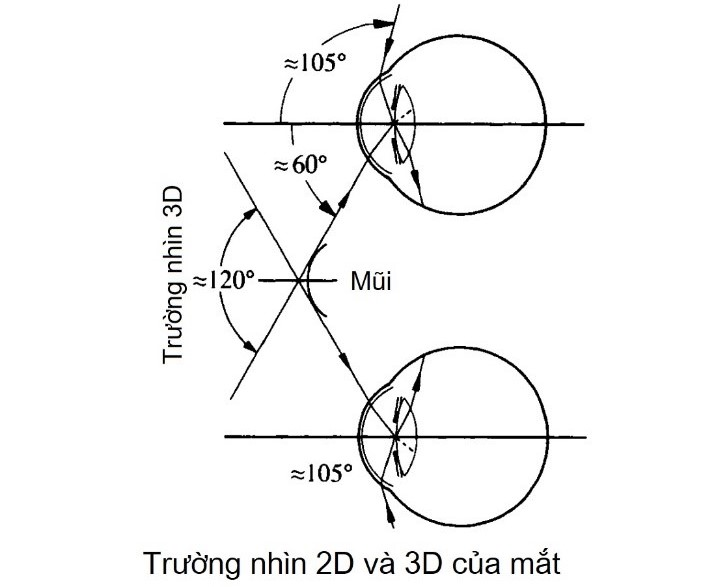
\includegraphics[width= 1\linewidth]{9}
		\caption{\small\textit{\color{timhieukhoahoc}Hình $9$. Trường nhìn $2$D và $3$D của mắt.}}
		\vspace*{-10pt}
	\end{figure}
	$\pmb{10.}$ \textbf{\color{timhieukhoahoc}Chộp hình tốc độ cao.}
	\vskip 0.1cm 
	Nhờ có cơ vận nhãn mắt người có thể chộp hình rất nhanh, tức là bắt lấy đối tượng cần chú ý. Tốc độ chộp hình mắt người là $700$ độ/giây, mắt máy khó so được. 
	\vskip 0.1cm
	Mắt người và động vật có đặc tính hướng quang, tức là hướng tới nguồn sáng chói nhất xuất hiện, sau đó mới tránh đi.  
	\vskip 0.1cm
	$\pmb{11.}$ \textbf{\color{timhieukhoahoc}Lưu ảnh võng mạc.}
	\vskip 0.1cm
	Hiện tượng lưu ảnh trong võng mạc làm giảm khả năng quan sát những vật chuyển động nhanh, nhưng lại làm cho hình ảnh chuyển động rời rạc trở thành liên tục. Trong phòng tối, thời gian lưu ảnh lâu hơn, chỉ cần $24$ hình/giây bạn thấy chuyển động là liên tục. Nhưng khi xem TV và nhìn màn vi tính, ít nhất màn hình phải chớp $50$ hình/giây mới không thấy nhấp nháy.  
	\vskip 0.1cm
	$\pmb{12.}$ \textbf{\color{timhieukhoahoc}Xử lý bậc cao.} Mắt nhìn và truyền tín hiệu thị giác về cho não bộ để xử lý ở bậc cao hơn, thông qua các bước:
	\vskip 0.1cm
	$1$. \textit{Thấy} là cảm thụ, nhận biết.
	\vskip 0.1cm
	$2$. \textit{Làm} là ra quyết định và đáp ứng. 
	\vskip 0.1cm
	$3$. \textit{Biết} là trải nghiệm và hồi tưởng thị giác.
	\vskip 0.1cm
	Thông thường, bạn chỉ thấy những cái bạn muốn thấy, và bỏ qua những cái khác.  
	\vskip 0.1cm
	$\pmb{13.}$ \textbf{\color{timhieukhoahoc}Thấy to hay nhỏ.}
	\vskip 0.1cm Hãy quan sát Hình $10$, hình tròn đen nào to? 
	\begin{figure}[H]
		\vspace*{-5pt}
		\centering
		\captionsetup{labelformat= empty, justification=centering}
		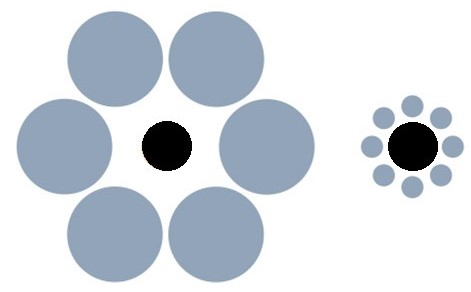
\includegraphics[width= 1\linewidth]{10}
		\caption{\small\textit{\color{timhieukhoahoc}Hình $10$. So sánh kích thước hình tròn đen.}}
		\vspace*{-10pt}
	\end{figure}
	Bây giờ bạn hãy đo kiểm tra: chẳng hình tròn đen nào to hơn cả! 
	\vskip 0.1cm
	Cái thấy là so sánh thôi! để cạnh vật to thấy nhỏ, để cạnh vật nhỏ thấy to? Để cạnh vật tối thấy sáng, để cạnh vật sáng thấy tối. Màu sắc cũng bị ảnh hưởng tương tự bởi màu của các vật bên cạnh và xuất hiện trước đó.  
	\vskip 0.1cm
	\textbf{\color{timhieukhoahoc}Chiếu sáng bảo vệ mắt}
	\vskip 0.1cm
	$\pmb{14.}$ \textbf{\color{timhieukhoahoc}Ô nhiễm ánh sáng.}
	\vskip 0.1cm
	Ngày nay, các bệnh không lây nhiễm như đột quỵ, tai biến, ung thư, béo phì, tiểu đường, hiếm muộn được biết đến là nguyên nhân gây tử vong hàng đầu. Tất cả điều liên quan trực tiếp hoặc gián tiếp đến ô nhiễm môi trường ánh sáng. 
	\begin{figure}[H]
		\vspace*{-5pt}
		\centering
		\captionsetup{labelformat= empty, justification=centering}
		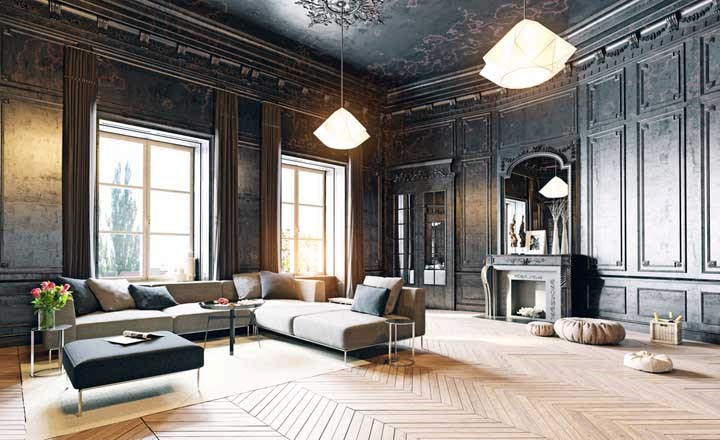
\includegraphics[width= 1\linewidth]{11}
		\caption{\small\textit{\color{timhieukhoahoc}Hình $11$. Chiếu sáng nội thất ô nhiễm.}}
		\vspace*{-10pt}
	\end{figure}
	Sự khác biệt của môi trường chiếu sáng nhân tạo với chiếu sáng tự nhiên về lượng sáng, phân bố, cấu trúc phổ, chói lóa và nhịp điệu là tác nhân gây ô nhiễm. Giải pháp phù hợp nhất cho chiếu sáng nhân tạo, lấy con người làm trung tâm (HCL) là giả lập bầu trời tự nhiên.   
	\vskip 0.1cm
	$\pmb{15.}$ \textbf{\color{timhieukhoahoc}Chiếu sáng SkyLighting.} 
	\vskip 0.1cm
	Là tên gọi giải pháp chiếu sáng nâng cao thị lực, bảo vệ mắt và sức khỏe.
	Bản chất của SkyLighting là giả lập ánh sáng bầu trời tự nhiên, sử dụng đèn SkyLED, lựa chọn màu trần, tường phù hợp và điều khiển thông minh. 
	\begin{figure}[H]
		\vspace*{-5pt}
		\centering
		\captionsetup{labelformat= empty, justification=centering}
		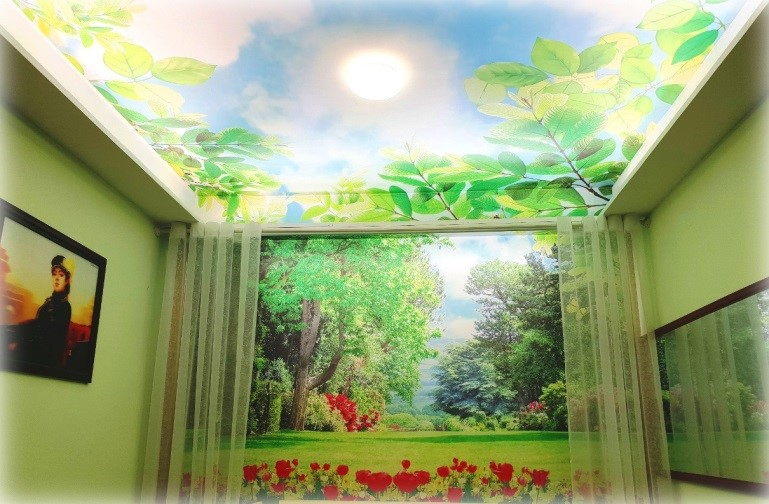
\includegraphics[width= 1\linewidth]{12}
		\caption{\small\textit{\color{timhieukhoahoc}Hình $12$. Hình ảnh SkyLighting nội thất.}}
		\vspace*{-10pt}
	\end{figure}
	Một ví dụ SkyLighting trên Hình $10$ sử dụng $8$ đèn SkyLED giả lập bầu trời, $1$ đèn ốp trần giả lập mặt trời và $1$ đèn chiếu tranh giả lập cửa sổ. Ánh sáng thay đổi cường độ và nhiệt độ màu theo nhịp ngày đêm với độ rọi $900$ lux vào buổi trưa. 
	\vskip 0.1cm
	$\pmb{16.}$ \textbf{\color{timhieukhoahoc}Hạn chế nguy cơ ánh sáng xanh.}
	\vskip 0.1cm
	\vskip 0.1cm
	Ngày nay, thời gian làm việc với màn hình công nghệ rất dài nên cần có giải pháp hạn chế ánh sáng xanh. Tuy nhiên, các nghiên cứu cho thấy, chỉ cần bảo vệ tế bào nón tập trung ở vùng hoàng điểm. 
	\vskip 0.1cm
	Giải pháp hạn chế ánh sáng xanh bằng cách chuyển sang chế độ ánh sáng vàng chỉ giảm bớt được khoảng $30\%$ lượng ánh sáng xanh, nhưng lại gây buồn ngủ. 
	\vskip 0.1cm
	Nghiên cứu của chúng tôi cho thấy, bật đèn chiếu sáng xung quanh màn hình sẽ giảm độ chói của hình ảnh rơi vào vùng hoàng điểm $4$ lần, như được minh họa trên Hình $13$. Đó là vì đường đồng tử co lại khi chiếu sáng vùng ngoại vi. Hơn nữa khi bật đèn, thị lực tăng lên và người dùng còn tỉnh táo hơn.
	\begin{figure}[H]
		\vspace*{-5pt}
		\centering
		\captionsetup{labelformat= empty, justification=centering}
		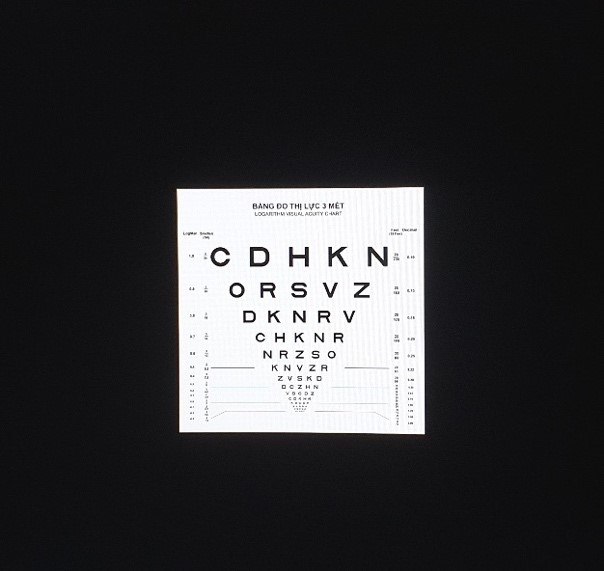
\includegraphics[width= 1\linewidth]{13a}
		
		\vspace*{2pt}
		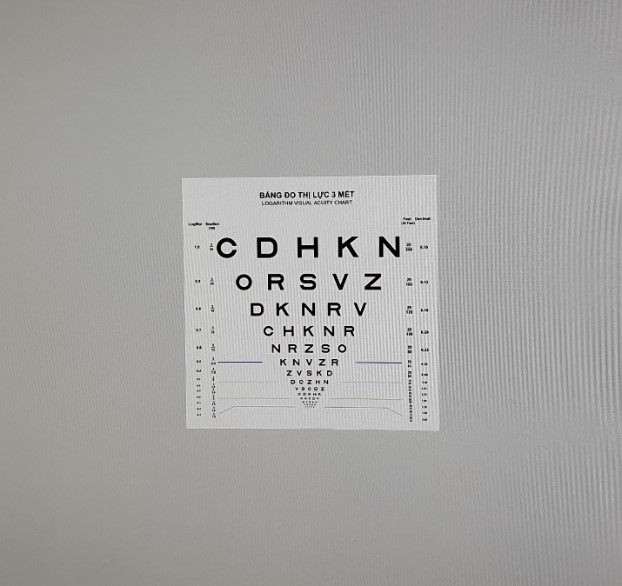
\includegraphics[width= 1\linewidth]{13b}
		\caption{\small\textit{\color{timhieukhoahoc}Hình $13$. Ảnh chụp bảng thử mắt dưới $2$ điều kiện chiếu sáng xung quanh.}}
		\vspace*{-10pt}
	\end{figure}
	$\pmb{18.}$ \textbf{\color{timhieukhoahoc}Lời khuyên cho người dùng màn hình.} 
	\vskip 0.1cm
	Khi phải làm việc nhiều với màn hình công nghệ, để giảm lượng ánh sáng xanh rơi vào hoàng điểm, cần phải tăng lượng sáng xung quanh màn hình bằng cách tăng độ rọi, và/hoặc sử dụng các màu sáng cho nền tường phía sau màn hình.
	\vskip 0.1cm
	Không được tắt đèn khi xem TV, khi dùng màn hình điện tử, tránh dùng mặt bàn hoặc quần áo sẫm màu.
	\vskip 0.1cm
	$\pmb{19.}$ \textbf{\color{timhieukhoahoc}Bảo vệ mắt khi ra ngoài trời.}
	\vskip 0.1cm
	Ánh sáng ngoài trời rất mạnh và chứa nhiều tia cực tím. Ra ngoài cần đeo kính râm cắt hết tia cực tím và giảm ít nhất $5$ lần tia khả kiến. Các bạn cận thị không dùng kính cận râm sẽ bị đục thủy tinh thể và giác mạc do tia cực tím, hỏng võng mạc do ánh sáng xanh. 
	\vskip 0.1cm
	$\pmb{20.}$ \textbf{\color{timhieukhoahoc}Tật cận thị với vòng xoáy bẩn.}
	\vskip 0.1cm
	Tật cận thị ngày càng phổ biến với nguyên nhân trực tiếp là nhìn gần quá nhiều, trong môi trường ánh sáng yếu.
	\begin{figure}[H]
		\vspace*{-5pt}
		\centering
		\captionsetup{labelformat= empty, justification=centering}
		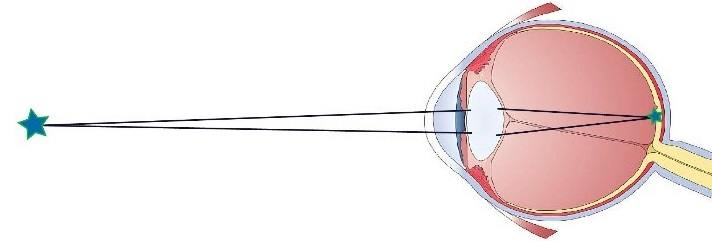
\includegraphics[width= 1\linewidth]{14}
		\caption{\small\textit{\color{timhieukhoahoc}Hình $14$. Nhãn cầu dài do áp lực nhìn gần.}}
		\vspace*{-10pt}
	\end{figure}
	Khi nhìn gần nhiều, hình ảnh hội tụ sau võng mạc tạo áp lực làm nhãn cầu dài ra, không hồi phục được nữa (Hình $14$). Nếu bạn đeo kính cận $-2$ D (f=$0{,}5$ m), khi không đeo kính, bạn vẫn nhìn rõ trong khoảng cách nhỏ hơn $50$ cm. Tuy nhiên, khi đeo kính để nhìn màn hình ở khoảng cách $O=0{,}4$ m, hình ảnh sẽ thu gần lại theo công thức Gauss: 
	\begin{align*}
		O&=i*O/(f+O) \\
		&= 0{,}4*0{,}5/(0,4+0,5) = 0,22 (m).
	\end{align*}
	Khoảng cách $0{,}22$ m là yếu tố kích thích độ cận lên tới $-4{,}5$ D, nếu bạn sử dụng màn hình thường xuyên. Đó là lý do tại sao từ ngày đeo kính thường xuyên, bạn tăng số liên tục.
	\vskip 0.1cm
	Giải pháp phù hợp là, bạn phải bỏ kính ra khi làm việc gần. Bạn phải đeo kính giảm $2$ số khi bạn đọc sách. 
	\vskip 0.1cm
	$\pmb{21.}$ \textbf{\color{timhieukhoahoc}Chiếu sáng lớp học.}
	\vskip 0.1cm
	Tiêu chuẩn TCVN--$7118$ của Việt nam quy định độ rọi mặt bàn học sinh $300$ lux, mặt bảng $500$ lux và hệ số chói lóa UGR < $19$. Phần lớn các lớp học ở Việt nam không đạt được $2$ tiêu chuẩn sau và là một trong các nguyên nhân tăng nguy cơ mắc tật khúc xạ.
	\begin{figure}[H]
		\vspace*{5pt}
		\centering
		\captionsetup{labelformat= empty, justification=centering}
		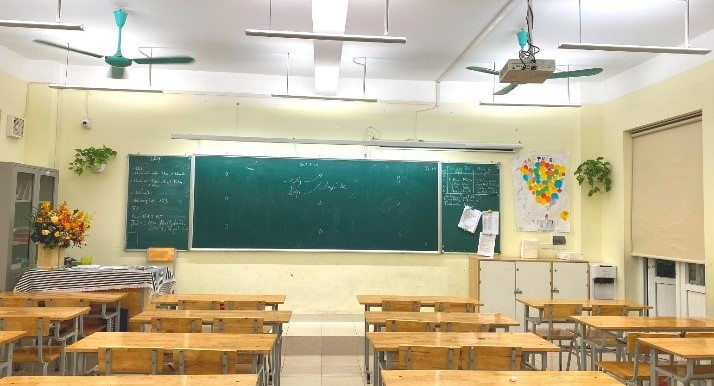
\includegraphics[width= 1\linewidth]{15}
		\caption{\small\textit{\color{timhieukhoahoc}Hình $15$. Chiếu sáng lớp học SkyLighting.}}
		\vspace*{-10pt}
	\end{figure}
	Mô hình do đề tài cấp Nhà nước ĐTĐLCN.$30/18$ xây dựng đã đáp ứng vượt mức tất cả các tiêu chuẩn quốc gia và quốc tế về chiếu sáng lớp học, sử dụng hệ thống SkyLED và đèn chiếu bảng, đã được cấp nhiều bằng sáng chế (Hình $15$).
	\vskip 0.1cm
	$\pmb{22.}$ \textbf{\color{timhieukhoahoc}Bàn học ở nhà.}
	\vskip 0.1cm
	Nguy cơ mắc tật khúc xạ của học sinh ở nhà còn cao hơn trên lớp, vì bạn không nhìn bảng. Hộp sáng SkyBox giả lập bầu trời trên Hình $16$ tạo ra môi trường sáng gần với bầu trời, độ rọi cao, đồng đều, không chói lóa. 
	\begin{figure}[H]
		\vspace*{-5pt}
		\centering
		\captionsetup{labelformat= empty, justification=centering}
		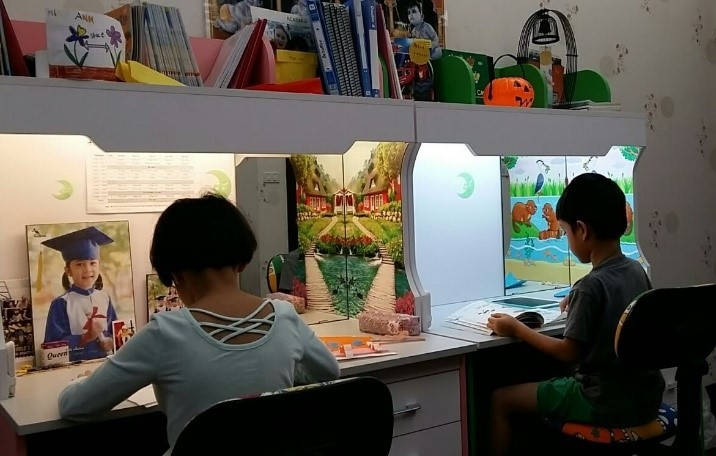
\includegraphics[width= 1\linewidth]{16}
		\caption{\small\textit{\color{timhieukhoahoc}Hình $16.$ Bàn học với hộp sáng Skybox.}}
		\vspace*{-5pt}
	\end{figure}
	Ánh sáng tán xạ góc khối rộng hơn $\pi sr$ sẽ xóa hết bóng đổ. Nền sáng phía sau không những làm tăng thị lực, mà còn bảo vệ vùng điểm vàng do đồng tử thu hẹp. 
	\vskip 0.1cm
	\textbf{\color{timhieukhoahoc}Kết luận:}
	\vskip 0.1cm
	Môi trường chiếu sáng định hình hệ thống thị giác của chúng ta. Chúng ta cũng đang thay đổi môi trường chiếu sáng. Sử dụng giải pháp chiếu sáng SkyLighting và thay đổi hành vi sẽ nâng cao hiệu quả học tập và chất lượng cuộc sống. 
\end{multicols}



